\documentclass[xcolor=dvipsnames]{beamer}

\title[Modeling using Matchgates]{Generative Modeling using Matchgate Circuits}
\author{Peter Luo, Hong Ye Hu, Susanne F. Yelin}

\date{\today} 

\usetheme{Boadilla}
\usecolortheme{seahorse}
\useoutertheme[subsection=false]{miniframes}  
\useinnertheme{circles}

\definecolor{logoBlue}{HTML}{003278}
\definecolor{blueDark}{HTML}{a3b6d4}
\definecolor{blueLight}{HTML}{e7eef8}
\definecolor{grey}{HTML}{b1b5b8}

\setbeamercolor*{palette tertiary}{bg=blueDark}
\setbeamercolor{frametitle}{fg=black,bg=blueLight}
\setbeamercolor{normal text}{fg=black,bg=white}

\usefonttheme{professionalfonts}
\usepackage{newpxtext}
\renewcommand\familydefault{\rmdefault}
\usepackage{amsmath}
\usepackage{bm}
\usepackage{tikz}
\usepackage{tikz-cd}
\tikzcdset{scale cd/.style={every label/.append style={scale=#1},
    cells={nodes={scale=#1}}}}
\usetikzlibrary{quantikz}
\usepackage{graphicx}

\DeclareMathOperator*{\E}{\mathbb{E}}
\newcommand{\set}[1]{\left\{#1\right\}}

\begin{document}

\frame{\titlepage}

\section{Generative Modeling}

\begin{frame}{How Neural Networks Learn}
  
  \begin{itemize}
    \item Define a \textcolor{red}{loss function} $L(\bm{\theta})$ which captures how close the network's output is to the desired output
  \end{itemize}

  \begin{figure}
    \centering
    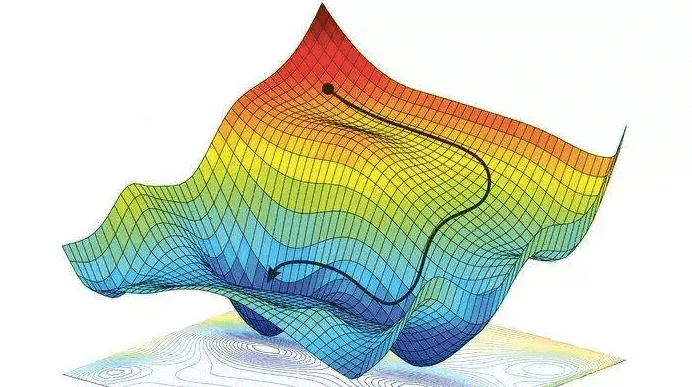
\includegraphics[width=0.5\textwidth]{gd.png}
  \end{figure}

  \begin{itemize}
    \item We can use optimization algorithms to adjust $\bm{\theta}$ to get closer to the minimum of $L$ 
    \item Automatic differentiation is what allows modern ML models to learn
  \end{itemize}

\end{frame}

\begin{frame}{Generative Modeling}

    \begin{itemize}
      \item Rather than doing a classification or prediction task, generative models strive to generate more instances of their training data
      \item Examples: ChatGPT, DALL-E, Synthetic Data Generation 
    \end{itemize}
    \begin{figure}
      \centering
          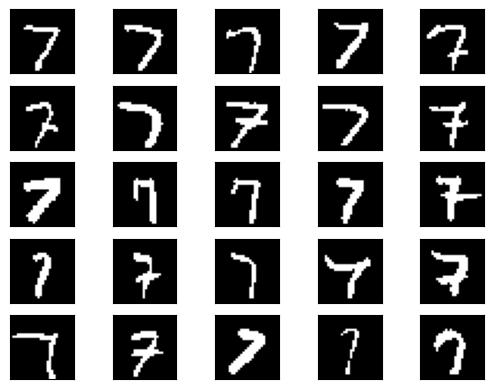
\includegraphics[width=0.4\textwidth]{MNIST.png}
      \end{figure}

\end{frame}

\begin{frame}
  \frametitle{Parametrized Quantum Circuits}
  \begin{itemize}
    \item Quantum gates can be \textcolor{red}{parametrized}
    \item By replacing the neural network with a parametrized quantum circuit and then measuring its output, we obtain a \textcolor{red}{hybrid} quantum-classical system compatible with machine learning procedures
  \end{itemize}
  \begin{figure}
    \centering
    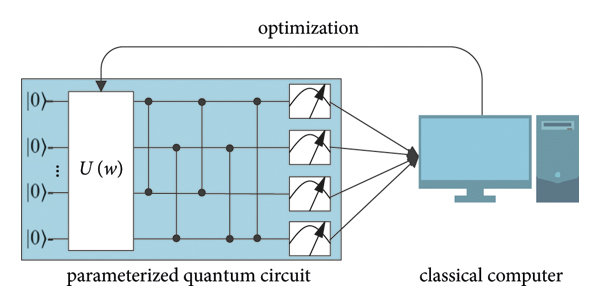
\includegraphics[width=0.7\textwidth]{pqc.png}
  \end{figure}
\end{frame}

\begin{frame}{Quantum Circuits as Generative Models}
  \begin{itemize}
    \item Parametrized quantum circuits (PQC) can be used as generative models
    \item Not a lot is known about how PQCs perform on such tasks, especially at large scale
    \item Solution: Matchgate circuits
    \item Continuously parametrized, efficiently simulatable
  \end{itemize}
\end{frame}

\begin{frame}
  \begin{itemize}
    \item \textcolor{red}{Goal:} To run a Matchgate circuit on generative tasks involving 49+ qubits
    \item Assess the generative capability of Matchgate circuits
    \item Test theoretical results pertaining to the large-qubit or overparametrized regime
  \end{itemize}
\end{frame}

\begin{frame}{Generative Adversarial Networks (GAN)}

  \begin{itemize}
    \item Consists of two networks $G_{\bm{\theta}}$ and $D_{\bm{\phi}}$ with parameters $\bm{\theta}$ and $\bm{\phi}$ and their own loss functions $L_G(\bm{\theta},\bm{\phi})$ and $L_D(\bm{\theta},\bm{\phi})$
    \item $G_{\bm{\theta}}:\{0,1\}^{28\times 28}\to\{0,1\}^{28\times 28}$ and $D_{\bm{\phi}}:\{0,1\}^{28\times 28}\to [0,1]$
  \end{itemize}

  \begin{figure}
    \centering
    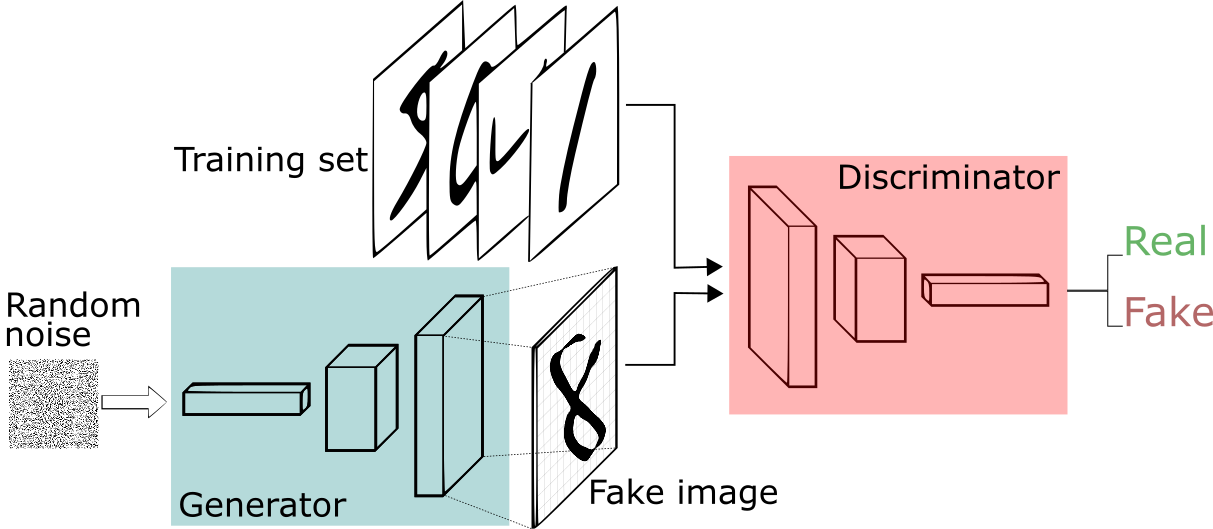
\includegraphics[width=0.7\textwidth]{GANs.png}
  \end{figure}

\end{frame}

\begin{frame}

  \begin{itemize}
    \item Real data $\bm{y}_1,\ldots,\bm{y}_n$ comes from an underlying probability distribution $p_{\text{real}}$
    \item The output of $G_{\bm{\theta}}$ are samples $\bm{x}_1,\ldots,\bm{x}_n$ from $p_{\bm{\theta}}$
    \item The loss functions are 
    \begin{align*}
      L_G(\bm{\theta},\bm{\phi})&=-\E_{\bm{x}\sim p_{\bm{\theta}}}\left[\log(D_{\bm{\phi}}(\bm{x}))\right]\\
      L_D(\bm{\theta},\bm{\phi})&=-\left(\E_{\bm{y}\sim p_{\text{real}}}\left[\log(D_{\bm{\phi}}(\bm{y}))\right]+\E_{\bm{x}\sim p_{\bm{\theta}}}\left[\log(1-D_{\bm{\phi}}(\bm{x}))\right]\right).
    \end{align*}
    \item Approximate with sample means in practice
  \end{itemize}

\end{frame}
  

\section{Matchgate Circuits}

\begin{frame}{Valiant's Definition}
  \begin{itemize}
    \item Matchgates were first introduced by Valiant (2001)
    \item For a given undirected weighted graph $G$ where $V(G)=[n],$ define the \textcolor{red}{Pfaffian} to be
    \[\text{Pf}(B)=\sum_{\substack{\text{perfect matchings} \\ M}}\text{sgn}(M)\prod_{(ij)\in M}w_{ij},\]
    where $B$ is the adjacency matrix of $G$
    \begin{center}
      \includegraphics[width=0.8\textwidth]{perfmatch.jpg}
    \end{center}
  \end{itemize}
\end{frame}

\begin{frame}
  \begin{itemize}
    \item Define the \textcolor{red}{Pfaffian sum} to be 
    \[\text{PfS}(B)=\sum_{A\subseteq [n]}\left(\prod_{i\in A}x_i\right)\text{Pf}(B[A])\]
    \item Pfaffian sums are just Pfaffians:
    \[\text{PfS}(B)=
    \begin{cases}
      \text{Pf}(B+\Lambda_n) & n\text{ even}\\
      \text{Pf}(B^++\Lambda_{n+1}) & n\text{ odd}
    \end{cases}\]
    \item Theorem (Cayley): $\text{Pf}(B)^2=\text{Det}(B)$
    \item Pfaffians are computable in polynomial time
    \item Matchgates are Pfaffian sums where we set some $x_i$ to 1 and all others to 0
  \end{itemize}
\end{frame}

\begin{frame}{Matchgate Speedup}
  \begin{itemize}
    \item For a Matchgate circuit $C,$ 
    \[|\bra{\underline{y}}C\ket{\underline{x}}|^2=|\text{PfS}(M_{\underline{x},\underline{y}})|^2.\]
    \item Valiant: Computing Pfaffians and Pfaffian Sums are fast
    \item Terhal and DiVincenzo (2001): There is a correspondence to noninteracting fermions, and computing determinants is fast
  \end{itemize}
\end{frame}

\begin{frame}{Majorana Basis}
  \begin{itemize}
    \item We can also understand Matchgate circuits in the context of free fermions. 
    \item Given $n$ fermionic modes with creation operators $c_1^\dagger,\ldots,c_n^\dagger,$ the \textcolor{red}{Majorana operators} $\gamma_1,\ldots,\gamma_{2n}$ are 
    \[\gamma_{2j-1}=c_j+c_j^\dagger,\qquad\gamma_{2j}=-i(c_j-c_j^\dagger)\]
    for $j=1,\ldots,n$ and satisfy the anticommutation relation
    \[\{\gamma_p,\gamma_q\}=2\delta_{pq}I.\]
  \end{itemize}
\end{frame}

\begin{frame}{Jordan-Wigner Transformation}
  \begin{itemize}
    \item Spin Hamiltonians (i.e. a collection of $n$ qubits) are the same as fermionic Hamiltonians
    \item We use
    \[\gamma_{2i-1}=\prod_{j=1}^{i-1}(-Z_j)X_i,\qquad\gamma_{2i}=-\prod_{j=1}^{i-1}(-Z_j)Y_i\]
    \item Products of two Majoranas look like
    \[I\otimes\cdots\otimes I\otimes U_1\otimes Z\otimes\cdots\otimes Z\otimes U_2\otimes I\otimes\cdots\otimes I\]
    where $U_1,U_2\in\{X,Y\}$
  \end{itemize}
\end{frame}

\begin{frame}{Defining Matchgates}
  \begin{itemize}
    \item Matchgates are a class of parametrized quantum gates, generated by 
    $$e^{-iX\otimes X\theta/2},~e^{-iY\otimes Y\theta/2},~e^{-iX\otimes Y\theta/2},~e^{-iY\otimes X\theta/2},~e^{-iIZ\theta/2},~e^{-iZI\theta/2}$$
    \item All of the exponents are products of Majoranas.
    \item Matchgates are \textcolor{red}{differentiable} with respect to $\theta$ and can be simulated in \textcolor{red}{polynomial time} 
  \end{itemize}

  \begin{figure}
    \centering
    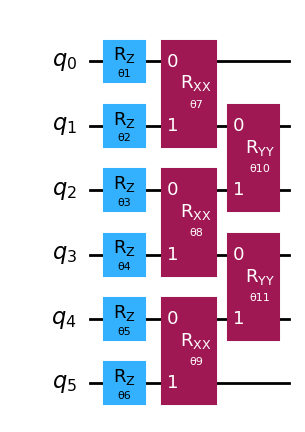
\includegraphics[width=0.2\textwidth]{output.png}
  \end{figure}
\end{frame}

\section{Gradients}
\begin{frame}{Computing Gradients}
  \begin{itemize}
    \item To get to the minimum of a loss function, we need to compute its gradient.
    \item Parameter-Shift Rule: If $L(\bm{\theta})=\bra{0}U_\theta^\dagger AU_\theta\ket{0}$ where $U_\theta=e^{-ia\theta G}$ and $G^2=I,$ then
    \[\frac{\partial L}{\partial\bm{\theta}_i}=r\left(L\left(\bm{\theta}+\frac{\pi}{4r}\vec{\bf{e}}_i\right)+L\left(\bm{\theta}-\frac{\pi}{4r}\vec{\bf{e}}_i\right)\right)\]
    \item To find the gradient of $L_G(\bm{\theta},\bm{\phi}),$ just need to compute the value of $L_G$ at various points.
  \end{itemize}
\end{frame}

\begin{frame}{Parameter Shift in Practice}
  \begin{itemize}
    \item Denote ${\bm{\theta}}^+=\bm{\theta}+\frac{\pi}{4r}\vec{\bf{e}}_i$ and ${\bm{\theta}}^-=\bm{\theta}+\frac{\pi}{4r}\vec{\bf{e}}_i.$ We have
    \begin{align*}
      \frac{\partial L}{\partial\bm{\theta}_i}&=r\left(L\left(\bm{\theta}+\frac{\pi}{4r}\vec{\bf{e}}_i\right)+L\left(\bm{\theta}-\frac{\pi}{4r}\vec{\bf{e}}_i\right)\right)\\
      &\approx r\left(-\frac{1}{N}\sum_{\ell=1}^N\log(D_{\bm{\phi}}(G_{{\bm{\theta}}^+}(z^{(\ell)})))-\frac{1}{N}\sum_{\ell=1}^N\log(D_{\bm{\phi}}(G_{{\bm{\theta}}^-}(z^{(\ell)})))\right)
    \end{align*}
    \item For each parameter $\theta_i,$ we need to \textcolor{red}{change the parameters} of the quantum circuit, then \textcolor{red}{sample $2N$ times} 
  \end{itemize}

\end{frame}

\begin{frame}{Gradient of $L_D$}
  \begin{align*}
    \nabla_{\bm{\phi}} L_D({\bm{\theta}},{\bm{\phi}})&=\nabla_{\bm{\phi}}\left(-\left(\E_{\bm{y}\sim p_{\text{real}}}\left[\log(D_{\bm{\phi}}(\bm{y}))\right]+\E_{\bm{x}\sim p_{\bm{\theta}}}\left[\log(1-D_{\bm{\phi}}(\bm{x}))\right]\right)\right)\\
    &=-\left(\E_{\bm{y}\sim p_{\text{real}}}\left[\nabla_{\bm{\phi}}\log(D_{\bm{\phi}}(\bm{y}))\right]+\E_{\bm{x}\sim p_{\bm{\theta}}}\left[\nabla_{\bm{\phi}}\log(1-D_{\bm{\phi}}(\bm{x}))\right]\right)
  \end{align*}
  \begin{itemize}
    \item Mathematically, we can interchange the gradient and the summation/integral
    \item Most ML packages (e.g. Flux.jl) can do autodifferentiation
  \end{itemize}
\end{frame}

\begin{frame}{Gradient of $L_G$}
  \begin{align*}
    \nabla_{\bm{\theta}} L_G({\bm{\theta}},{\bm{\phi}})&=\nabla_{\bm{\theta}}\left(-\E_{\bm{x}\sim p_{\bm{\theta}}}\left[\log(D_{\bm{\phi}}(\bm{x}))\right]\right)\\
    &=-\nabla_{\bm{\theta}}\sum_{x\in\set{0,1}^n}\log(D_{\bm{\phi}}(x))p_{\bm{\theta}}(x)\\
    &=-\sum_{x\in\set{0,1}^n}\log(D_{\bm{\phi}}(x))\nabla_{\bm{\theta}} p_{\bm{\theta}}(x)
\end{align*}
\begin{itemize}
  \item It's not as easy to differentiate $p_{\bm{\theta}}(x)$
\end{itemize}
\end{frame}

\begin{frame}{REINFORCE Trick}
  \begin{itemize}
    \item Rewrite $\nabla_{\bm{\theta}}p_{\bm{\theta}}(x)=p_{\bm{\theta}}(x)\nabla_{\bm{\theta}}\log p_{\bm{\theta}}(x)$
  \end{itemize}
  \begin{align*}
    -\sum_{x\in\set{0,1}^n}\log(D_{\bm{\phi}}(x))\nabla_{\bm{\theta}} p_{\bm{\theta}}(x)&=-\sum_{x\in\set{0,1}^n}\log(D_{\bm{\phi}}(x))p_{\bm{\theta}}(x)\nabla_{\bm{\theta}}\log p_{\bm{\theta}}(x)\\
    &=-\E_{x\sim p_{\bm{\theta}}}\left[\log(D_{\bm{\phi}}(x))\nabla_{\bm{\theta}}\log p_{\bm{\theta}}(x)\right]\\
    &\approx -\frac{1}{N}\sum_{\ell=1}^N\log(D_{\bm{\phi}}(x^{(\ell)}))\nabla_{\bm{\theta}}\log p_{\bm{\theta}}(x^{(\ell)})
  \end{align*}
\end{frame}

\begin{frame}{Analytical Log Gradient}
  \begin{itemize}
    \item Analytical algorithm to compute $\nabla_{\bm{\theta}}\log p_{\bm{\theta}}(x)$ for a given $x=x_1x_2\ldots x_n\in\set{0,1}^n$
    \item Rather than sampling all bits at one time, we are sampling \textcolor{red}{bit-by-bit}
    \item Mathematically, $\displaystyle\log p_{\bm{\theta}}(x)=\log p_{\bm{\theta}}(x_1)+\sum_{j=2}^n\log p_{\bm{\theta}}(x_j|x_1\ldots x_{j-1})$
    \item $U_{\bm{\theta}}\ket{0}$ is a \textcolor{red}{Gaussian state} and is thus uniquely defined by a covariance matrix $M(\bm{\theta})$ with entries $M_{pq}(\bm{\theta})=\frac{i}{2}\bra{0}U_{\bm{\theta}}^\dagger|[\gamma_p,\gamma_q]|U_{\bm{\theta}}\ket{0}$
    \item $p_{\bm{\theta}}(x_i)=\frac12(1+(-1)^{x_i}M_{2i-1,2i}({\bm{\theta}}))$
  \end{itemize}
\end{frame}

\begin{frame}{Updating the Covariance Matrix}
  \begin{itemize}
    \item Wick's Theorem: Upon measuring the $i$th qubit and obtaining a measurement outcome $x_i,$ the covariance matrix transforms as
    \[M_{pq}^{x_i}(\bm{\theta})=M_{pq}(\bm{\theta})+\frac{(-1)^{x_i}}{2p_{\bm{\theta}}(x_i)}(M_{2i-1,q}(\bm{\theta})M_{2i,p}(\bm{\theta})-M_{2i-1,p}(\bm{\theta})M_{2i,q}(\bm{\theta}))\]
    \item Subsequently, $p_{\bm{\theta}}(x_j|x_i)=\frac12(1+(-1)^{x_j}M_{2j-1,2j}^{x_i}(\bm{\theta}))$
    \item All relevant information are stored in the \textcolor{red}{covariance matrix}
    \item We can compute $\nabla_{{\bm{\theta}}}M_{pq}({\bm{\theta}})$ efficiently
  \end{itemize}
\end{frame}

\begin{frame}{Computing the Log Gradient}
  \begin{itemize}
    \item Only need to keep track of two $2n\times 2n$ matrices
  \end{itemize}
  \[\begin{tikzcd}[scale cd=0.75]
	\begin{array}{c} \begin{bmatrix}& & \\&M_{pq}(\bm{\theta})&\\&&\end{bmatrix} \end{array} & \begin{array}{c} \begin{bmatrix}& & \\&\nabla_{\bm{\theta}} M_{pq}(\bm{\theta})&\\&&\end{bmatrix} \end{array} & \shortstack{$p_{\bm{\theta}}(x_1)$ \\ $\nabla_{\bm{\theta}} p_{\bm{\theta}}(x_1)$} \\
	\begin{array}{c} \begin{bmatrix}& & \\&M_{pq}^{x_1}({\bm{\theta}})&\\&&\end{bmatrix} \end{array} & \begin{array}{c} \begin{bmatrix}& & \\&\nabla_{\bm{\theta}} M_{pq}^{x_1}({\bm{\theta}})&\\&&\end{bmatrix} \end{array} & \shortstack{$p_{\bm{\theta}}(x_2|x_1)$ \\ $\nabla_{\bm{\theta}} p_{\bm{\theta}}(x_2|x_1)$} \\
	\vdots & \vdots \\
	\begin{array}{c} \begin{bmatrix}& & \\&M_{pq}^{x_1,x_2,\ldots,x_{n-1}}({\bm{\theta}})&\\&&\end{bmatrix} \end{array} & \begin{array}{c} \begin{bmatrix}& & \\&\nabla_{\bm{\theta}} M_{pq}^{x_1,x_2,\ldots,x_{n-1}}({\bm{\theta}})&\\&&\end{bmatrix} \end{array} & \shortstack{$p_{\bm{\theta}}(x_n|x_1,\ldots,x_{n-1})$ \\ $\nabla_{\bm{\theta}} p_{\bm{\theta}}(x_n|x_1,\ldots,x_{n-1})$}
	\arrow[from=1-2, to=1-3]
	\arrow[from=2-2, to=2-3]
	\arrow[from=4-2, to=4-3]
\end{tikzcd}\]
\end{frame}

\begin{frame}{Code}
  \begin{itemize}
    \item Written in Julia, using Yao and FLOYao packages
    \item Utilized FLOYao package to harness Matchgate optimizations
  \end{itemize}
\end{frame}

\begin{frame}{Runtime Comparison}
  \begin{center}
    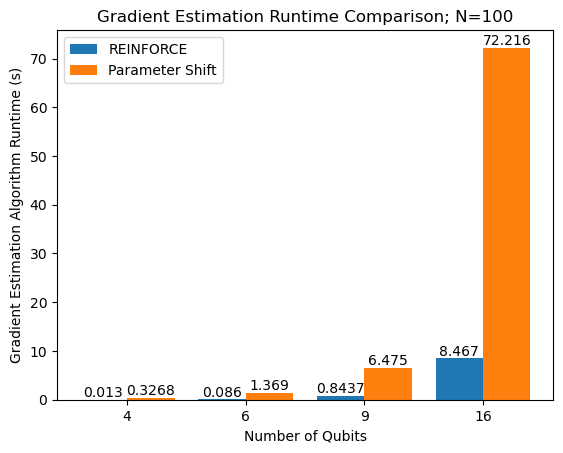
\includegraphics[width=0.7\textwidth]{runtimecomparison.png}
  \end{center}
\end{frame}
\section{Putting it all together}

\begin{frame}{Setup}
  \begin{enumerate}
    \item Use a parametrized Matchgate circuit for $G$
    \item Use a classical neural network for $D$
    \item Use the GAN loss functions and train
  \end{enumerate}
  \begin{figure}
    \centering
    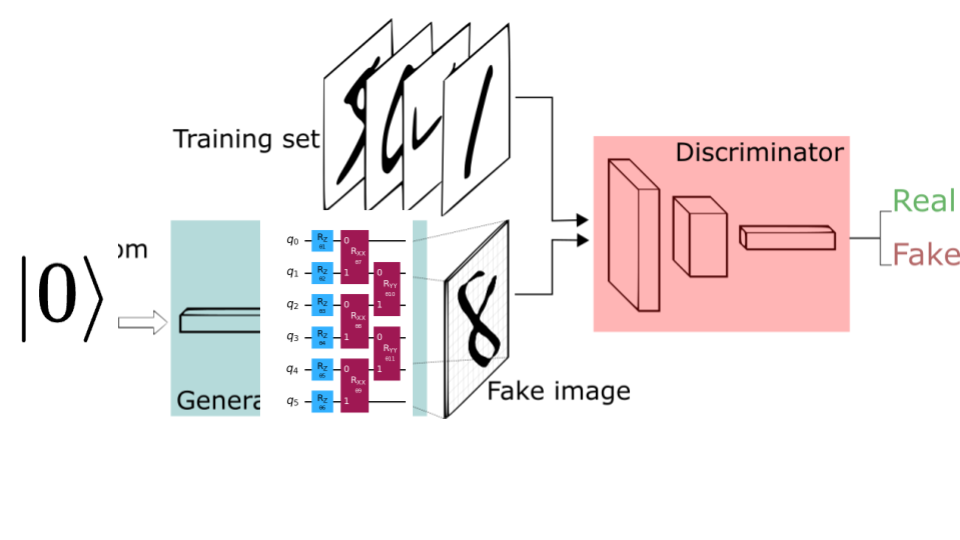
\includegraphics[width=0.7 \textwidth]{Untitled presentation (1).png}
  \end{figure}
\end{frame}

\begin{frame}{Acknowledgements}
  \begin{itemize}
    \item Hong-Ye Hu and Susanne Yelin  
    \item Yelin group undergrads: Jorge, Fiona, Victoria, and Kevin
  \end{itemize}
\end{frame}

\begin{frame}{Questions?}
  \begin{itemize}
    \item Thanks for listening!
  \end{itemize}
\end{frame}

\section{Appendix}
\begin{frame}{Pfaffians}
  \begin{itemize}
    \item Define the \textcolor{red}{Pfaffian sum} to be 
    \[\text{PfS}(B)=\sum_{A\subseteq [n]}\left(\prod_{i\in A}x_i\right)\text{Pf}(B[A])\]
    \item Pfaffian sums are just Pfaffians:
    \[\text{PfS}(B)=
    \begin{cases}
      \text{Pf}(B+\Lambda_n) & n\text{ even}\\
      \text{Pf}(B^++\Lambda_{n+1}) & n\text{ odd}
    \end{cases}\]
    where
    \[\Lambda_n=
    \begin{pmatrix}
      0 & x_1x_2 & -x_1x_3 & \cdots\\
      -x_1x_2 & 0 & x_2x_3 & \cdots\\
      x_1x_3 & -x_2x_3 & \ddots & \\
      \vdots & \vdots & & 
    \end{pmatrix}\]
  \end{itemize}
\end{frame}

\begin{frame}{Matchgate Definition}
  \begin{itemize}
    \item A \textcolor{red}{matchgate} $\Gamma$ is $(G,X,Y,T)$ where $G$ is a graph and $X,Y,T$ partition the vertices. For $Z\subseteq X\cup Y,$ define 
    \[\chi(\Gamma,Z)=\mu(\Gamma,Z)\text{PfS}(G-Z)\]
    where $\mu(\Gamma,Z)\in\{-1,1\}$ and $x_i=1$ if $i\in T,~x_i=0$ otherwise.
    \item The \textcolor{red}{character matrix} $\chi(\Gamma)$ is the $2^{|X|}\times 2^{|Y|}$ matrix with 
    \[\chi(\Gamma)_{i,j}=\chi(\Gamma,X_i\cup Y_j).\]
    \item Defined in this way, not all matchgates are unitary
    \item Take the ones that are unitary and interpret them as quantum gates
  \end{itemize}
  
\end{frame}

\begin{frame}{REINFORCE Full Derivation}
  \begin{align*}
    \nabla_\theta L_G(\theta,\phi)&=-\nabla_\theta\E_{x\sim p_\theta}\left[\log(D_\phi(x))\right]\\
    &=-\nabla_\theta\sum_{x\in\set{0,1}^n}\log(D_\phi(x))p_\theta(x)\\
    &=-\sum_{x\in\set{0,1}^n}\log(D_\phi(x))\nabla_\theta p_\theta(x)\\
    &=-\sum_{x\in\set{0,1}^n}\log(D_\phi(x))p_\theta(x)\nabla_\theta\log p_\theta(x)\\
    &=-\E_{x\sim p_\theta}\left[\log(D_\phi(x))\nabla_\theta\log p_\theta(x)\right]\\
    &\approx -\frac{1}{N}\sum_{\ell=1}^N\log(D_\phi(x^{(\ell)}))\nabla_\theta\log p_\theta(x^{(\ell)})
  \end{align*}
\end{frame}

\begin{frame}{Probability Derivation}
  Recall that for fermionic creation and annihilation operators, we have 
  \begin{itemize}
    \item The number operator: $n_j=c_j^\dagger c_j$
    \item Squaring to zero: $c_jc_j=c_j^\dagger c_j^\dagger=0$
    \item Anticommutation relation $\{c_j^\dagger,c_k\}=\delta_{jk}$
    \item Definition of Majorana: $\gamma_{2j-1}=c_j+c_j^\dagger,~\gamma_{2j}=-i(c_j-c_j^\dagger)$
    \item Claim: $\langle n_j\rangle=\frac12(1-\frac{i}{2}\langle [\gamma_{2j-1},\gamma_{2j}]\rangle)$
  \end{itemize}
\end{frame}

\end{document}